\documentclass[11pt,a4paper]{article}

% Packages
\usepackage[utf8]{inputenc}
% T1 fontenc removed: basic TeX Live has no cm-super, so T1 text was rendered as bitmap Type 3 fonts.
\PassOptionsToPackage{hyphens}{url}
\usepackage{amsmath,amssymb,amsthm}
\usepackage{mathtools}
\usepackage{graphicx}
\usepackage{booktabs}
% Hyperlinks (disable duplicate anchor names)
\usepackage[hypertexnames=false]{hyperref}
% \usepackage{cleveref}  % Not available in basic TeX Live
% \usepackage{algorithm}  % Not needed
% \usepackage{algorithmic}  % Not needed
% \usepackage{natbib}  % Not available in basic TeX Live
\usepackage{geometry}
\usepackage{float}
% \usepackage{subcaption}  % Not available in basic TeX Live
% \usepackage{xcolor}  % Not available in basic TeX Live

% Minimal reference helpers (cleveref not available in basic TeX Live).
% We infer the reference type from the label prefix (e.g., fig:..., thm:..., sec:...).
\makeatletter
\def\Cref@getprefix#1:#2\relax{#1}
\def\Cref@prefix@sec{sec}
\def\Cref@prefix@fig{fig}
\def\Cref@prefix@tab{tab}
\def\Cref@prefix@eq{eq}
\def\Cref@prefix@thm{thm}
\def\Cref@prefix@prop{prop}
\def\Cref@prefix@lem{lem}
\def\Cref@prefix@cor{cor}
\def\Cref@prefix@conj{conj}
\def\Cref@prefix@def{def}
\def\Cref@prefix@rem{rem}
\def\Cref@prefix@ex{ex}

\def\Cref@type@cap#1{%
  \edef\Cref@tmp{#1}%
  \ifx\Cref@tmp\Cref@prefix@sec Section%
  \else\ifx\Cref@tmp\Cref@prefix@fig Figure%
  \else\ifx\Cref@tmp\Cref@prefix@tab Table%
  \else\ifx\Cref@tmp\Cref@prefix@eq Equation%
  \else\ifx\Cref@tmp\Cref@prefix@thm Theorem%
  \else\ifx\Cref@tmp\Cref@prefix@prop Proposition%
  \else\ifx\Cref@tmp\Cref@prefix@lem Lemma%
  \else\ifx\Cref@tmp\Cref@prefix@cor Corollary%
  \else\ifx\Cref@tmp\Cref@prefix@conj Conjecture%
  \else\ifx\Cref@tmp\Cref@prefix@def Definition%
  \else\ifx\Cref@tmp\Cref@prefix@rem Remark%
  \else\ifx\Cref@tmp\Cref@prefix@ex Example%
  \else Ref.%
  \fi\fi\fi\fi\fi\fi\fi\fi\fi\fi\fi\fi
}

\def\Cref@type@low#1{%
  \edef\Cref@tmp{#1}%
  \ifx\Cref@tmp\Cref@prefix@sec section%
  \else\ifx\Cref@tmp\Cref@prefix@fig figure%
  \else\ifx\Cref@tmp\Cref@prefix@tab table%
  \else\ifx\Cref@tmp\Cref@prefix@eq equation%
  \else\ifx\Cref@tmp\Cref@prefix@thm theorem%
  \else\ifx\Cref@tmp\Cref@prefix@prop proposition%
  \else\ifx\Cref@tmp\Cref@prefix@lem lemma%
  \else\ifx\Cref@tmp\Cref@prefix@cor corollary%
  \else\ifx\Cref@tmp\Cref@prefix@conj conjecture%
  \else\ifx\Cref@tmp\Cref@prefix@def definition%
  \else\ifx\Cref@tmp\Cref@prefix@rem remark%
  \else\ifx\Cref@tmp\Cref@prefix@ex example%
  \else ref.%
  \fi\fi\fi\fi\fi\fi\fi\fi\fi\fi\fi\fi
}

\DeclareRobustCommand{\Cref}[1]{%
  \begingroup
  \edef\Cref@label{#1}%
  \edef\Cref@prefix{\expandafter\Cref@getprefix\Cref@label:\relax}%
  \hyperref[#1]{\Cref@type@cap{\Cref@prefix}~\ref*{#1}}%
  \endgroup
}
\DeclareRobustCommand{\cref}[1]{%
  \begingroup
  \edef\Cref@label{#1}%
  \edef\Cref@prefix{\expandafter\Cref@getprefix\Cref@label:\relax}%
  \hyperref[#1]{\Cref@type@low{\Cref@prefix}~\ref*{#1}}%
  \endgroup
}
\makeatother

\geometry{margin=0.9in}
\setlength{\emergencystretch}{2em} % reduce overfull lines without \sloppy
\setlength{\textfloatsep}{10pt plus 2pt minus 2pt}
\setlength{\intextsep}{8pt plus 2pt minus 2pt}
\setlength{\abovecaptionskip}{4pt}
% captions in \small
\makeatletter
\long\def\@makecaption#1#2{\vskip\abovecaptionskip\small\sbox\@tempboxa{#1: #2}\ifdim\wd\@tempboxa>\hsize #1: #2\par\else\global\@minipagefalse\hb@xt@\hsize{\hfil\box\@tempboxa\hfil}\fi\vskip\belowcaptionskip}
\makeatother
% Float placement parameters (reduce float-page waste)
\renewcommand{\topfraction}{0.9}
\renewcommand{\bottomfraction}{0.6}
\renewcommand{\textfraction}{0.07}
\renewcommand{\floatpagefraction}{0.85}
\setcounter{topnumber}{3}
\setcounter{totalnumber}{5}

% Theorem environments
\theoremstyle{plain}
\newtheorem{theorem}{Theorem}[section]
\newtheorem{lemma}[theorem]{Lemma}
\newtheorem{proposition}[theorem]{Proposition}
\newtheorem{corollary}[theorem]{Corollary}
\newtheorem{conjecture}[theorem]{Conjecture}

\theoremstyle{definition}
\newtheorem{definition}[theorem]{Definition}
\newtheorem{example}[theorem]{Example}

\theoremstyle{remark}
\newtheorem{remark}[theorem]{Remark}

% Custom commands
\newcommand{\R}{\mathbb{R}}
\newcommand{\Z}{\mathbb{Z}}
\newcommand{\N}{\mathbb{N}}


\title{\textbf{Magic Gems: A Polyhedral Framework for Magic Squares}}

\author{Kyle Elliott Mathewson\\
\textit{Faculty of Science, University of Alberta}\\
\texttt{kyle.mathewson@ualberta.ca}}

\date{}

\begin{document}

\maketitle

\begin{abstract}
A magic square can be read as an arrangement of vectors from the centroid whose vertical components cancel along every row, column and both diagonals.
The \emph{Magic Gem} of an $n\times n$ magic square is the convex hull of the tips $\mathbf p_{ij}=(x_{ij},y_{ij},z_{ij})$ of these vectors, where $(x_{ij},y_{ij})$ is the centred cell and $z_{ij}$ the centred entry.
We show that $\sum\mathbf p_{ij}=\mathbf 0$ for every arrangement, so unweighted vector balance is not specific to magic squares; the magic-specific consequences are the height-weighted moments $\sum z\,\varphi(x)=\sum z\,\varphi(y)=0$, which include Loly's invariant, while $\sum z\,xy$ is not forced.
For order four we compute the $880$ gems exactly ($8$ to $16$ vertices, $39$ $f$-vectors, $352$ combinatorial types, $155$ volumes, $616$ congruence classes) and, by an exact computer-assisted calculation, determine all their isometry groups: the $48$ associative squares give centrally symmetric gems, the $304$ remaining self-complementary squares give gems with exactly one half-turn symmetry, and the other $528$ gems have none; every gem is chiral except the $48$ centrally symmetric ones.
Every gem lies in a box that depends only on $n$, certain corner and side-extreme points are always vertices, and the $880$ gems have $554$ distinct Ehrhart polynomials.
We also prove, with computer assistance, that the Siamese square of every odd order $n\ge5$ has a gem with exactly twelve vertices.
\medskip

\noindent\textbf{Keywords:} magic squares, convex polyhedra, symmetry, combinatorial geometry, moment of inertia
\end{abstract}

\section{Introduction}
\label{sec:introduction}

Magic squares are among the oldest objects of recreational mathematics: the $3\times3$ Lo Shu belongs to Chinese tradition, a $4\times4$ square is engraved in D\"urer's \emph{Melencolia~I} (1514), and constructions for every order have been known for centuries \cite{andrews1960magic,pickover2002zen}.
The modern literature treats them from several directions: enumeration and the geometry of the polytopes whose lattice points are the squares \cite{stanley1973magic,ehrhart1973magic,ahmed2003polyhedral,beck2006insideout,beck2010enumeration}, spectral and matrix properties \cite{loly2009spectra,nordgren2012properties,nordgren2014spectra,cameron2013signatura}, and, in work of Loly and collaborators, physical invariants such as the moment of inertia and the multipole moments \cite{loly2004invariance,rogers2004inertia,rogers2005multipole}.

\begin{definition}[Magic square]
\label{def:magic_square}
An \emph{arrangement} of order $n$ is a bijection $S=(s_{ij})$ from the cells of the $n\times n$ grid onto $\{1,\dots,n^2\}$.
It is a \emph{magic square} if every row, every column and both main diagonals sum to the magic constant $M(n)=n(n^2+1)/2$, and \emph{semi-magic} if only the rows and columns do.
\end{definition}

\paragraph{The picture.}
Centre the grid at the origin and attach to the cell $(i,j)$ the vector
\[
\mathbf p_{ij}=(x_{ij},y_{ij},z_{ij}),
\]
whose horizontal part $(x_{ij},y_{ij})$ is the position of the cell and whose vertical part is the \emph{centred entry} $z_{ij}=s_{ij}-\frac{n^2+1}{2}$.
Then $S$ is magic exactly when the vertical components of these vectors cancel along every row, column and both diagonals (\Cref{lem:lines}; \Cref{fig:vectors}, \Cref{fig:lines}).
The \emph{Magic Gem} $\mathcal G(S)$ is the convex hull of the tips of the $n^2$ vectors $\mathbf p_{ij}$ (\Cref{sec:gem}).
\Cref{fig:vectors} shows the vectors of D\"urer's square and the gem they span; the tips are the gem's $12$ vertices and four strictly interior points, and $\sum\mathbf p_{ij}=\mathbf 0$.

\begin{figure}[htbp]
\centering
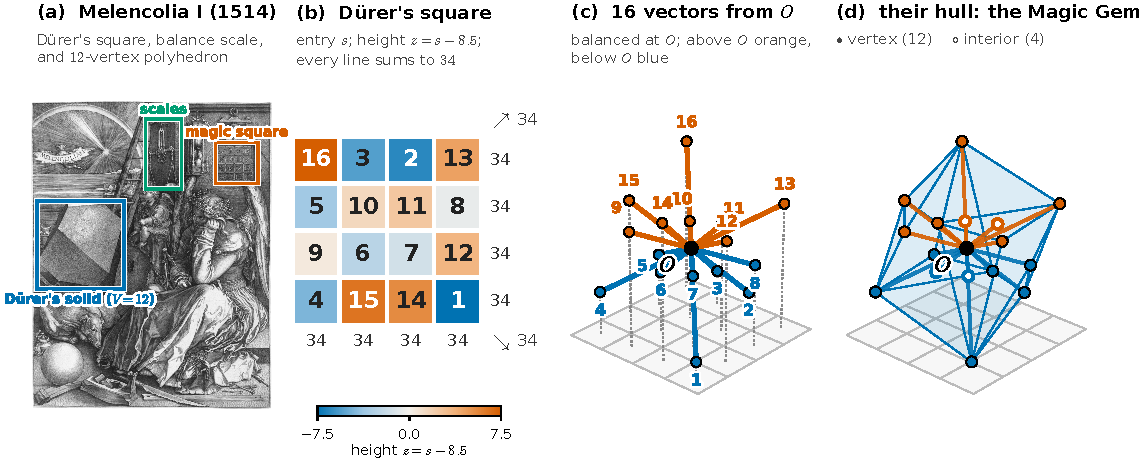
\includegraphics[width=\textwidth]{fig_vectors.pdf}
\caption{D\"urer's square as vectors from the centroid $O$. (a)~The square as a heat map of the heights $z_{ij}=s_{ij}-8.5$ (orange: above $O$, blue: below), with the entries $s_{ij}$ printed in the cells; every row, column and both diagonals sum to $34$. (b)~The $16$ vectors $\mathbf p_{ij}=(x_{ij},y_{ij},z_{ij})$: each points from $O$ over the cell $(x_{ij},y_{ij})$ of the floor grid (dotted drop lines) to a tip at height $z_{ij}$, labelled by the entry $s_{ij}$. (c)~The same vectors inside their convex hull, the Magic Gem: $12$ tips are vertices (filled dots) and $4$ are strictly interior (open dots). The colour bar is shared by (a) and (b). The vectors sum to $\mathbf 0$ for every arrangement of $1,\dots,16$ (\Cref{prop:centroid}); what singles out magic squares is how the heights cancel along lines (\Cref{fig:lines}).}
\label{fig:vectors}
\end{figure}

An interactive display of the $880$ order-four gems is available at \url{https://kylemath.github.io/MagicGemWebpage/}.

\paragraph{Results.}
\begin{enumerate}\setlength\itemsep{2pt}
\item \emph{Balance} (\Cref{sec:balance}). For every arrangement, magic or not, $\sum_{i,j}\mathbf p_{ij}=\mathbf 0$ (\Cref{prop:centroid}), so the unweighted statement ``the vectors balance about the centroid'' carries no information about $S$; it concerns all $n^2$ points, including those that are not vertices, not the solid hull.
The magic-specific statements weight each vector by its height: $\sum z\,\varphi(x)=\sum z\,\varphi(y)=0$ for every function $\varphi$ when $S$ is semi-magic, which contains the vanishing of the height-weighted centroid and Loly's invariant, while the mixed moment $\sum z\,xy$ is not forced (\Cref{prop:signed_mass}, \Cref{cor:loly}).
\item \emph{Symmetry of the order-four gems} (\Cref{sec:symmetry}). The complement $S\mapsto 17-S$ reflects the gem in the plane $z=0$. We prove that a self-complementary square yields a gem with an explicit isometry (a point reflection if $S$ is associative, a half-turn about a horizontal axis otherwise), and determine by exact computation the complete isometry group of each of the $880$ gems: $48$ gems are centrally symmetric, $304$ have exactly one half-turn symmetry, and $528$ have no symmetry (\Cref{thm:symmetry}). Facet orbits are classified (\Cref{prop:facet-orbits}).
\item \emph{Geometry of the $880$ gems} (\Cref{sec:gem-geometry-880}). Vertex counts, $f$-vectors, combinatorial types, volumes and congruence classes; the congruence classes are exactly the orbits of the complement map, and no two gems have the same vertex set.
Every gem lies in a fixed box, and the points over the corners and the extreme entries of each side are always vertices (\Cref{prop:box}); the order-four gems have $554$ distinct Ehrhart polynomials (\Cref{sec:ehrhart}).
\item \emph{Siamese gems} (\Cref{prop:siamese-12}). The Siamese square of every odd order $n\ge5$ has a gem with exactly twelve vertices, $26$ edges and $16$ facets (computer-assisted proof, \Cref{sec:app_siamese}); the fraction of points that are vertices tends to zero.
\end{enumerate}

\paragraph{What is and is not new.}
The polyhedral geometry of magic squares is classical: nonnegative integer matrices with all line sums equal to $t$ are the lattice points of the $t$-th dilate of the Birkhoff polytope, and their number is a polynomial in $t$ \cite{stanley1973magic,ehrhart1973magic,ziegler1995lectures}; the count of magic squares with distinct entries is an Ehrhart quasi-polynomial of an inside-out polytope \cite{beck2006insideout,beck2010enumeration}; the cones of magic squares and cubes have Hilbert-basis descriptions \cite{ahmed2003polyhedral}; contingency tables with fixed margins are the same lattice points seen as a sample space \cite{diaconis1995rectangular}.
In all of these the magic squares are the \emph{points} of a polytope, whereas the Magic Gem attaches a polyhedron to a \emph{single} square, in the spirit of the physical invariants of Loly and Rogers \cite{loly2004invariance,rogers2004inertia,rogers2005multipole} (see also \cite{loly2007franklin} for Franklin squares).
The balance statements of \Cref{sec:balance} are elementary and implicit in that work; we state and prove them in the gem's coordinates because the geometric picture invites misreadings of them.
The symmetry classification, the exact geometry of the $880$ gems (including the forced-vertex and Ehrhart statements) and the Siamese theorem are new.
The reading of the line conditions as orthogonality conditions on the height function, the hierarchy of moment conditions, the statistics of random arrangements and the enumeration of low-energy squares are developed in the companion paper \cite{mathewson_companion}; none of its results is used here.

\Cref{sec:gem} defines the gem, \Cref{sec:balance} treats balance, \Cref{sec:symmetry} symmetry, \Cref{sec:results} the exact geometry of the order-four and Siamese gems, \Cref{sec:discussion} open questions, and the appendices contain the computational methods and the remaining steps of the Siamese proof.

\section{The Magic Gem}
\label{sec:gem}

Let $S=(s_{ij})$ be an arrangement of order $n$, with cells indexed by $i,j\in\{0,\dots,n-1\}$ ($i$ the row from the top, $j$ the column from the left), and write $N=n^2$.

\begin{definition}[Gem coordinates and Magic Gem]
\label{def:gem_coords}
To the cell $(i,j)$ assign the point $\mathbf p_{ij}=(x_{ij},y_{ij},z_{ij})\in\R^3$ with
\begin{equation}
x_{ij}=j-\frac{n-1}{2},\qquad y_{ij}=\frac{n-1}{2}-i,\qquad z_{ij}=s_{ij}-\frac{N+1}{2}.
\label{eq:gem_coords}
\end{equation}
The \emph{Magic Gem} of $S$ is the convex hull $\mathcal G(S)=\operatorname{conv}\{\mathbf p_{ij}\}$.
The function $z=(z_{ij})$ is the \emph{height function} of $S$, and each $\mathbf p_{ij}$ is read as a vector from the origin.
Every centroid or moment statement in this paper refers to the full set of $N$ points $\mathbf p_{ij}$, including those that are not vertices, and not to the solid $\mathcal G(S)$.
\end{definition}

\paragraph{Terminology.}
Every point $\mathbf p_{ij}$ is of exactly one of three kinds: a \emph{vertex} (an extreme point of $\mathcal G(S)$); a \emph{strictly interior point} (lying in the topological interior of $\mathcal G(S)$); or a \emph{boundary non-vertex point} (lying on the boundary, in the relative interior of an edge or of a facet).
If $V,I,B$ denote their numbers, $V+I+B=N$ and the number of hull vertices is $V$; the $f$-vector is $(V,E,F)$.

The $x$-axis runs along the columns and the $y$-axis along the rows (top row at positive $y$); the centred entries have mean zero because the mean entry is $(N+1)/2$.
Let $x_j=j-\frac{n-1}2$ and $y_i=\frac{n-1}2-i$ denote the $n$ values taken by $x$ and $y$.
A \emph{line} is one of the $n$ rows, the $n$ columns, the main diagonal $\{i=j\}$ or the anti-diagonal $\{i+j=n-1\}$; each contains $n$ cells.
For a line $L$ let $\delta_L(S)=\sum_{c\in L}s_c-M(n)$ be its \emph{deviation}, so $S$ is magic iff $\delta_L(S)=0$ for all $2n+2$ lines.

\begin{lemma}[Means, variances, line vector sums]
\label{lem:lines}
For every arrangement $S$ of order $n$:
\begin{enumerate}
\item $\sum_{i,j}x_{ij}=\sum_{i,j}y_{ij}=\sum_{i,j}z_{ij}=0$ and $\sum_{i,j}x_{ij}y_{ij}=0$;
\item the empirical variances are $\operatorname{Var}(x)=\operatorname{Var}(y)=\frac{n^{2}-1}{12}$ and $\operatorname{Var}(z)=\frac{n^{4}-1}{12}$;
\item for every line $L$, $\delta_L(S)=\sum_{c\in L}z_c$, and
\[
\sum_{c\in L}\mathbf p_c=\bigl(n\,\bar x_L,\ n\,\bar y_L,\ \delta_L(S)\bigr),
\]
where $(\bar x_L,\bar y_L)$ is the centre of the line (the mean of its cell positions): $(0,y_i)$ for the row $i$, $(x_j,0)$ for the column $j$, and $(0,0)$ for both diagonals.
\end{enumerate}
In particular $S$ is magic if and only if the vector sum of the $\mathbf p_c$ along every line is horizontal, i.e.\ the vertical components cancel along every row, column and diagonal.
\end{lemma}

\begin{proof}
(1) $\sum_{i,j}x_{ij}=n\sum_j x_j=0$, likewise for $y$; $\sum z=\sum_{v=1}^{N}v-N\frac{N+1}2=0$; and $\sum xy=(\sum_jx_j)(\sum_iy_i)=0$.
(2) $\operatorname{Var}(x)=\frac1n\sum_jx_j^2$ is the variance of $n$ equally spaced points with unit spacing, $(n^2-1)/12$; the same holds for $y$, and for $z$ with $N$ points.
(3) Since $M(n)=n\frac{N+1}2$, $\sum_{c\in L}z_c=\sum_{c\in L}s_c-M(n)=\delta_L$. The cells of a row $i$ have $y=y_i$ and $x$ running over all $x_j$ (sum $0$); for a column the roles are exchanged; each diagonal is invariant under $(x,y)\mapsto(-x,-y)$, so its position sums vanish.
\end{proof}

\Cref{fig:lines} illustrates \Cref{lem:lines}(3) for D\"urer's square: along each of four lines the heights stack head to tail and return to zero, so the vector sum of the line is horizontal, $(0,6,0)=4\,(0,\tfrac32,0)$ for the top row; after swapping two entries the stack of the affected lines fails to close, by the deviation $\delta_L$.

\begin{figure}[htbp]
\centering
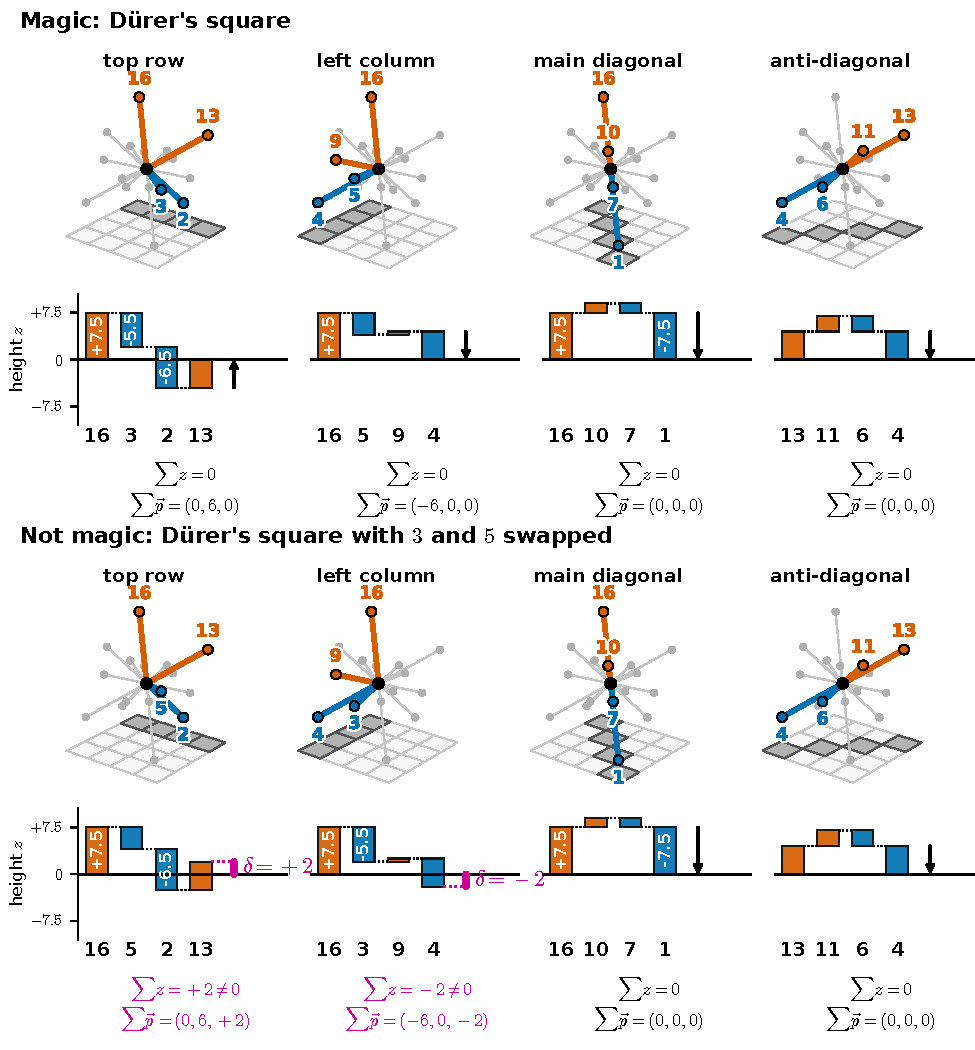
\includegraphics[width=0.92\textwidth]{fig_lines.pdf}
\caption{Magic means that heights cancel along every line. \emph{Top:} for D\"urer's square, the four vectors of the top row, left column, main diagonal and anti-diagonal (coloured, with their entries; the other twelve in grey; the cells of the line are shaded on the floor) and below each the heights $z=s-8.5$ of the line stacked head to tail in line order; the running total returns to $0$, so $\sum_{c\in L}\mathbf p_c$ is the horizontal vector $(n\bar x_L,n\bar y_L,0)$ of \Cref{lem:lines}(3), here $(0,6,0)$, $(-6,0,0)$, $\mathbf 0$, $\mathbf 0$. \emph{Bottom:} the same after swapping the entries $3$ and $5$, which is not magic: the top row and the left column no longer close (deviations $\delta_L=+2$ and $-2$, in magenta) and their vector sums acquire the vertical component $\delta_L$; the diagonals do not contain the swapped cells and still close.}
\label{fig:lines}
\end{figure}

\begin{example}[Lo Shu]
\label{ex:loshu}
For the Lo Shu square $S=\begin{pmatrix}2&7&6\\9&5&1\\4&3&8\end{pmatrix}$, $n=3$ and the centre value is $5$, so the nine points are
\[
\begin{array}{lll}
\mathbf p_{00}=(-1,1,-3), & \mathbf p_{01}=(0,1,2), & \mathbf p_{02}=(1,1,1),\\
\mathbf p_{10}=(-1,0,4), & \mathbf p_{11}=(0,0,0), & \mathbf p_{12}=(1,0,-4),\\
\mathbf p_{20}=(-1,-1,-1), & \mathbf p_{21}=(0,-1,-2), & \mathbf p_{22}=(1,-1,3).
\end{array}
\]
The top row has heights $-3+2+1=0$ and horizontal vector sum $(0,3,0)$.
The centre cell maps to the origin, which is the only non-vertex point and is strictly interior (\Cref{prop:centroid}); the gem has $f$-vector $(8,16,10)$ and volume $18$ (\Cref{fig:construction}).
\end{example}

\begin{proposition}[$D_4$-invariance]
\label{prop:symmetry_invariance}
Let $g\in D_4$ act on the grid and let $gS$ be the arrangement with $(gS)_c=s_{g^{-1}c}$.
Then $\mathcal G(gS)=\hat g\,\mathcal G(S)$, where $\hat g(x,y,z)=(g(x,y),z)$ is the isometry of $\R^3$ that applies the orthogonal map $g$ of the $(x,y)$-plane and fixes $z$; $\det\hat g=\det g$.
In particular $\mathcal G(gS)$ and $\mathcal G(S)$ are congruent, and the gem is an invariant of the $D_4$-orbit of $S$.
\end{proposition}

\begin{proof}
In the centred coordinates \eqref{eq:gem_coords}, each $g\in D_4$ acts on the cell positions as an orthogonal map of the plane (a rotation by a multiple of $90^\circ$ or a reflection in a coordinate axis or a diagonal), and $(x_{gc},y_{gc})=g(x_c,y_c)$.
The point of $gS$ over the cell $gc$ has height $(gS)_{gc}-\frac{N+1}2=z_c$.
Hence the point set of $gS$ is $\{(g(x_c,y_c),z_c)\}_c=\hat g\{\mathbf p_c\}_c$, and an affine bijection maps the convex hull of a set onto the convex hull of its image.
\end{proof}

Magic squares are mapped to magic squares by $D_4$ (lines go to lines), so every \emph{essentially different} magic square, that is, every $D_4$-orbit, has a single gem up to congruence.

\begin{figure}[htbp]
    \centering
    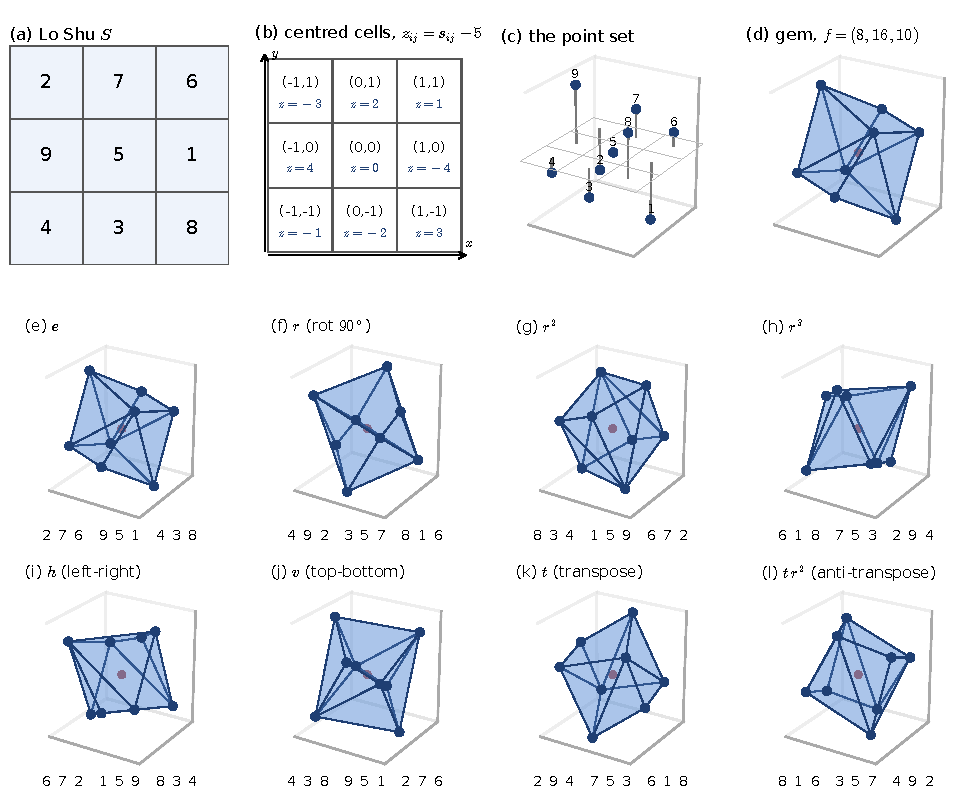
\includegraphics[width=\textwidth]{fig01_construction_d4.pdf}
    \caption{Construction of the Magic Gem and its $D_4$-invariance.
    Top row: (a)~the Lo Shu square $S$; (b)~the centred cells $(x_{ij},y_{ij})$ with the heights $z_{ij}=s_{ij}-5$; (c)~the nine points $\mathbf p_{ij}$ over the grid, labelled by the entries $s_{ij}$; (d)~their convex hull, the gem of \Cref{ex:loshu}, with $f$-vector $(8,16,10)$; the centre point $(0,0,0)$ is the only non-vertex point and is strictly interior.
    Rows two and three (e--l): the eight images of the Lo Shu under $D_4$---the identity $e$, the rotations $r,r^2,r^3$ by $90^\circ,180^\circ,270^\circ$, the left--right and top--bottom reflections $h,v$, and the two diagonal reflections (transpose $t$ and anti-transpose $tr^2$)---each printed row by row beneath its gem.
    All eight gems are drawn from the same viewpoint; by \Cref{prop:symmetry_invariance} they are the images of one another under the isometries $\hat g$, so they are congruent, and all have $f$-vector $(8,16,10)$ and volume $18$.}
    \label{fig:construction}
\end{figure}

\section{Balance: what the vectors from the centroid do and do not say}
\label{sec:balance}

\paragraph{Unweighted balance holds for every arrangement.}

\begin{proposition}[Centroid]
\label{prop:centroid}
For every arrangement $S$ of order $n$, $\sum_{i,j}\mathbf p_{ij}=\mathbf 0$: the origin is the centroid of the $N$ points, each of which is a vector from it. Moreover $\mathbf 0$ lies in the interior of $\mathcal G(S)$.
\end{proposition}

\begin{proof}
The sum vanishes by \Cref{lem:lines}(1). The centroid of a finite point set that is not contained in a plane is an interior point of its convex hull, as a convex combination with all weights positive; the points $\mathbf p_{ij}$ span $\R^3$ since the positions $(x_{ij},y_{ij})$ do and the heights are not all equal for $n\ge2$.
\end{proof}

This is a consequence of centring the coordinates and carries no information about $S$; in particular it does not distinguish magic squares from arbitrary arrangements.
It is a statement about the point set with unit weights, and not about the solid: the hull depends only on its vertex set, points that are not vertices do not affect it, and the centre of mass of the solid $\mathcal G(S)$ need not be the origin (for $829$ of the $880$ gems of order four it is not).
The hull records the extent of the point set (extreme points, faces, volume), not how the heights are distributed over the cells.

\paragraph{Height-weighted balance is what magic means.}
Take the \emph{signed mass} $m_{ij}=z_{ij}$ at the planar position $(x_{ij},y_{ij})$, with total mass $0$.
Write $\rho_i=\sum_jz_{ij}$ and $\gamma_j=\sum_iz_{ij}$ for the row and column mass sums; by \Cref{lem:lines}(3) they are the row and column deviations of $S$.

\begin{proposition}[Height-weighted moments]
\label{prop:signed_mass}
Let $S$ be an arrangement of order $n\ge3$.
\begin{enumerate}
\item $S$ is semi-magic if and only if $\rho_i=0$ for every row and $\gamma_j=0$ for every column.
\item For every function $\varphi\colon\R\to\R$,
\[
\sum_{i,j}z_{ij}\,\varphi(x_{ij})=\sum_j\varphi(x_j)\gamma_j,\qquad
\sum_{i,j}z_{ij}\,\varphi(y_{ij})=\sum_i\varphi(y_i)\rho_i .
\]
Hence if $S$ is semi-magic, $\sum z\,\varphi(x)=\sum z\,\varphi(y)=0$ for every $\varphi$ (for $\varphi(t)=t^k$, all $k\ge0$; for $k=1$ the height-weighted centroid is the origin).
Conversely, if $\sum z\,\varphi(x)=\sum z\,\varphi(y)=0$ for all $\varphi$, then $S$ is semi-magic.
\item The mixed moment is not forced: for $n=4$ there are magic squares with $\sum z\,xy\neq0$.
\end{enumerate}
\end{proposition}

\begin{proof}
(1) By \Cref{lem:lines}(3), a row sums to $M(n)$ if and only if its heights sum to $0$; likewise for columns.
(2) Grouping the cells by column, $\sum_{i,j}z_{ij}\varphi(x_j)=\sum_j\varphi(x_j)\gamma_j$; the row identity is the same with $y_i,\rho_i$. If $\gamma=\rho=0$ both vanish. Conversely take $\varphi$ to be the indicator of a single value $x_{j_0}$ (the $x_j$ are distinct): then $\gamma_{j_0}=0$; likewise $\rho_{i_0}=0$, and (1) applies.
(3) Since $\sum xy=0$, $\sum z\,xy=\sum s\,xy=-P_{xy}$, the product of inertia of Loly's value-weighted planar body.
Exact enumeration over the $880$ essentially different magic squares of order $4$ gives $|P_{xy}|\in\{0,\dots,60\}$ with $48$ distinct values; it vanishes for $56$ classes and is non-zero for the other $824$.
\end{proof}

\Cref{fig:moments} shows both halves of \Cref{prop:signed_mass}. In panel~a the entries themselves are piles of checkers on a checkerboard, $s_{ij}$ checkers on cell $(i,j)$: every row and column carries $34$ checkers, so the horizontal centre of mass of all the checkers lies over the centre $O$ ($\sum s\,x=\sum s\,y=0$, which for $n=4$ is the height-weighted statement because $\sum x=\sum y=0$). Hence each column of heights has zero total mass and the lever of signed masses balances, while the mixed moment $\sum z\,xy$ takes the value $0$ for D\"urer's square and $+60$ for another magic square. The same weighted balance in vector form is \Cref{fig:weighted}.

\begin{figure}[htbp]
\centering
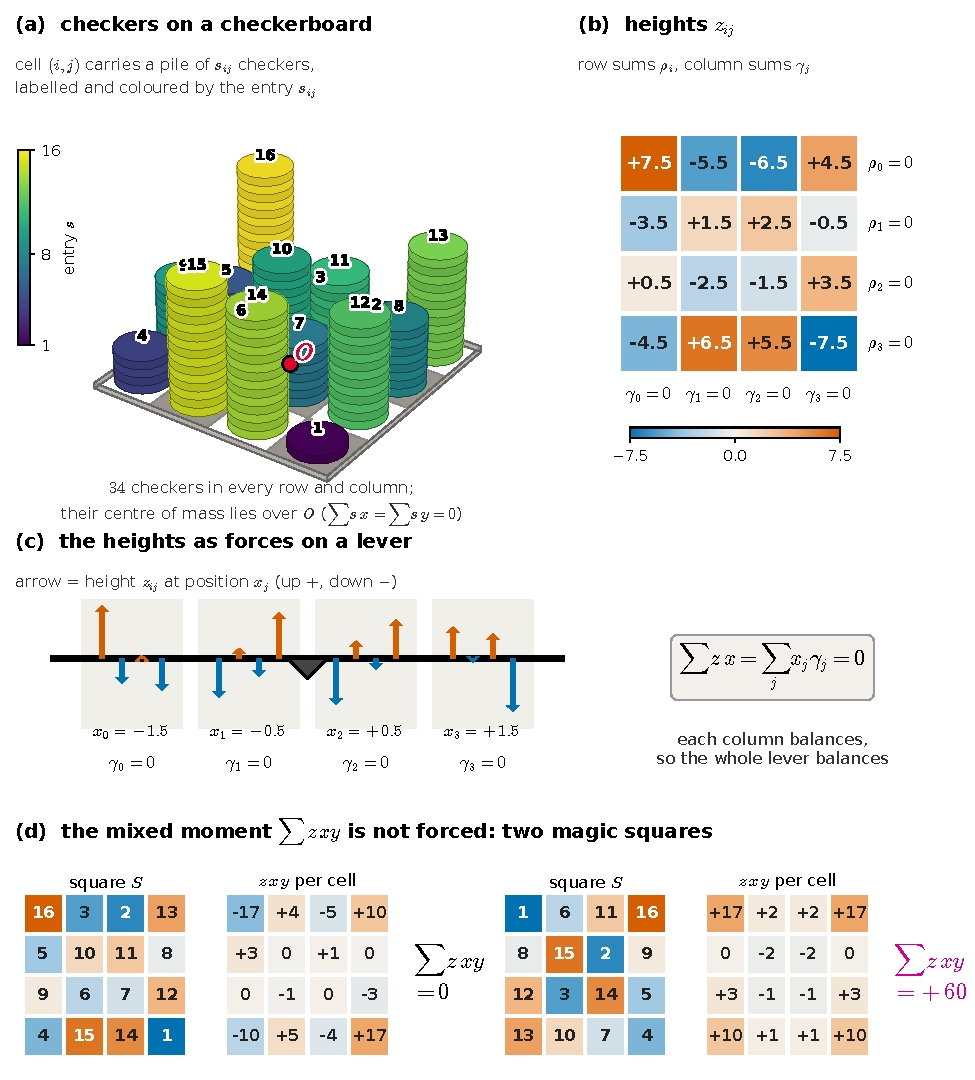
\includegraphics[width=0.8\textwidth]{fig_moments.pdf}
\caption{Height-weighted moments, order $n=4$. (a)~D\"urer's square as checkers on a $4\times4$ checkerboard, seen from the front: the pile on cell $(i,j)$ has $s_{ij}$ checkers (labelled, and coloured by the entry $s_{ij}$ with the colour bar shown); every row and column carries $34$ checkers, and the centre of mass of all the checkers lies over the board centre $O$ (red), $\sum s\,x=\sum s\,y=0$. (b)~The heights with row sums $\rho_i$ and column sums $\gamma_j$, all zero. (c)~Reading $z_{ij}$ as a force at position $x_j$ on a lever (up $+$, down $-$): every column has net force $\gamma_j=0$, hence $\sum z\,x=\sum_jx_j\gamma_j=0$ (\Cref{prop:signed_mass}(2)); the same holds for $y$ and the rows. (d)~The mixed moment is not forced: for two magic squares, the heights $z$ and the cell contributions $z\,x\,y$ (rounded to integers), which sum to $0$ for D\"urer's square and to $+60$ for the square $\begin{smallmatrix}1&6&11&16\\8&15&2&9\\12&3&14&5\\13&10&7&4\end{smallmatrix}$ (so $P_{xy}=-60$).}
\label{fig:moments}
\end{figure}

\begin{figure}[htbp]
\centering
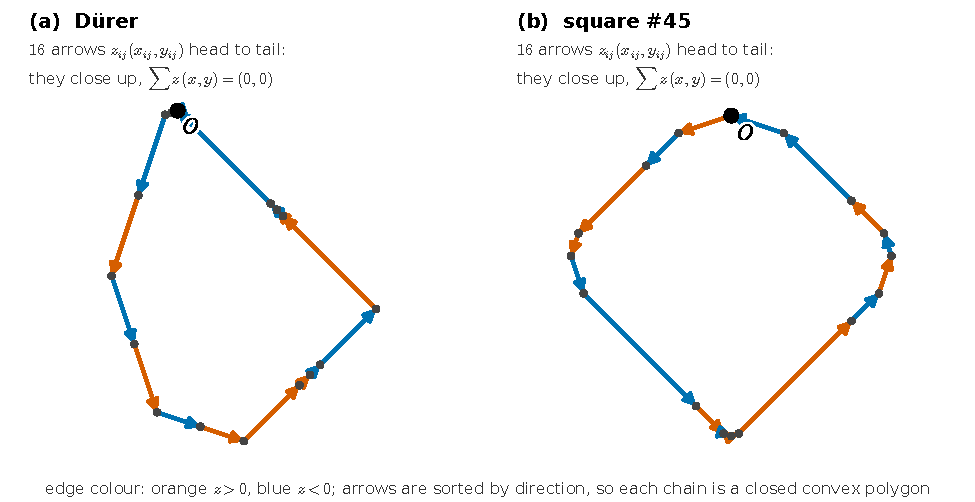
\includegraphics[width=0.9\textwidth]{fig_weighted_sum.pdf}
\caption{The height-weighted vector sum $\sum_{i,j}z_{ij}\,(x_{ij},y_{ij})=(0,0)$ for two magic squares: D\"urer's square and square \#45 of the $880$ (the second square of \Cref{fig:moments}d). The $16$ moment arms $z_{ij}(x_{ij},y_{ij})$ (orange for $z>0$, blue for $z<0$) are laid head to tail in order of direction; the chain closes at $O$ in both cases, which is $\sum z\,x=\sum z\,y=0$ (\Cref{prop:signed_mass}(2)). The right-hand tables give $\sum z\,xy$ for the four quadrants of the grid; they add to $0$ for D\"urer's square and to $+60$ for square \#45, so the weighted balance does not determine the mixed moment (\Cref{prop:signed_mass}(3)).}
\label{fig:weighted}
\end{figure}

Thus the height-weighted statements guaranteed by the line sums are exactly the pure axial ones: the vanishing of the first moment along each axis and Loly's invariant below.
The mixed moment can vanish for structural reasons: if $S$ is associative, $z$ is odd under $(x,y)\mapsto(-x,-y)$ (\Cref{sec:symmetry}) and $xy$ is even, so $\sum z\,xy=0$ (this accounts for the order-$3$ square and for $48$ of the $56$ vanishing classes of order $4$).

\begin{corollary}[Loly's moment of inertia]
\label{cor:loly}
For every arrangement, $I(S):=\sum_{i,j}s_{ij}(x_{ij}^2+y_{ij}^2)=\sum_jx_j^2\gamma_j+\sum_iy_i^2\rho_i+\frac{n^2(n^4-1)}{12}$.
In particular $I(S)=n^2(n^4-1)/12$ for every semi-magic square.
\end{corollary}

\begin{proof}
Substitute $s_{ij}=z_{ij}+\frac{N+1}2$. The first part is $\sum z\,(x^2+y^2)$, equal to $\sum_jx_j^2\gamma_j+\sum_iy_i^2\rho_i$ by \Cref{prop:signed_mass}(2); the second is $\frac{N+1}2\sum(x^2+y^2)=\frac{N+1}2\cdot2N\frac{n^2-1}{12}=\frac{n^2(n^4-1)}{12}$ by \Cref{lem:lines}(2).
\end{proof}

This is Loly's invariance \cite{loly2004invariance}, which he derived from the row and column sums.
For $n=3,\dots,9$ the value is $60,340,1300,3885,9800,21840,44280$.

\begin{remark}[Inertia tensor of the unit-mass point set]
\label{rem:inertia}
With unit masses at the $N$ points, the centre of mass is the origin and the inertia tensor about it is $I_{jk}=N(\delta_{jk}\operatorname{tr}\Sigma-\Sigma_{jk})$, where $\Sigma$ is the covariance matrix of the points \cite{goldstein2002classical}.
By \Cref{lem:lines} and \Cref{prop:signed_mass}(2), $I_{xx}=I_{yy}=n^{2}(n^{2}-1)(n^{2}+2)/12$, $I_{zz}=n^{2}(n^{2}-1)/6$, $I_{xy}=0$, $I_{xz}=-\sum_jx_j\gamma_j$ and $I_{yz}=-\sum_iy_i\rho_i$.
The diagonal entries are the same for all $N!$ arrangements and the tensor is diagonal for every semi-magic square, so the inertia of the unit-mass point set does not depend on the square.
The informative planar object is Loly's value-weighted body: its diagonal entries are fixed by the row and column sums (\Cref{cor:loly}), whereas the product of inertia $P_{xy}=-\sum s_{ij}x_{ij}y_{ij}$ is a mixed moment, fixed by no line sum; $D_4$ changes at most its sign.
\end{remark}

\begin{remark}[Covariance determinant]
\label{rem:detcov}
Let $\Sigma$ be the covariance matrix of $(x,y,z)$ over the $N$ points.
Since $\Sigma_{xy}=0$ and $\Sigma_{xx}=\Sigma_{yy}=:a$, $\Sigma_{zz}=:c$ are the same for all arrangements (\Cref{lem:lines}),
\[
\det\Sigma=a\,a\,c-a\,\Sigma_{xz}^2-a\,\Sigma_{yz}^2=a\bigl(ac-\Sigma_{xz}^2-\Sigma_{yz}^2\bigr),
\]
with $N\Sigma_{xz}=\sum z\,x$ and $N\Sigma_{yz}=\sum z\,y$.
So among all arrangements of order $n$ the determinant, which is proportional to the squared volume of the covariance ellipsoid, is largest exactly when $\sum z\,x=\sum z\,y=0$, in particular for every semi-magic square (\Cref{prop:signed_mass}(2) with $\varphi(t)=t$).
This concerns the point set, not its hull.
Numerically ($n=4$, $10^5$ uniformly random arrangements, \texttt{anc/vertex\_statistics.py}), the hull volume of a random arrangement has mean $75.7$ and is positively rank-correlated with $\det\Sigma$ (Spearman $0.65$), and the median of the $880$ magic gem volumes ($85.2$; mean $84.05$) lies at the $91$st percentile of the random volumes, numerical statements about samples only.
\end{remark}

\section{Symmetry of the gems}
\label{sec:symmetry}

Let $\rho(x,y,z)=(x,y,-z)$ be the reflection in the plane $z=0$.
The \emph{complement} of an arrangement is $\overline S=N+1-S$ (so $\overline S$ has height function $-z$), and $S$ is \emph{associative} if $S+r^2S=N+1$, where $r^2$ is the half-turn of the grid; $S$ is \emph{self-complementary} if $\overline S=gS$ for some $g\in D_4$.
Complements of magic squares are magic.

\begin{lemma}[Complement is a mirror image]
\label{lem:complement}
$\mathcal G(\overline S)=\rho\,\mathcal G(S)$.
If $\overline S=gS$ with $g\in D_4$, then $\iota_g:=\hat g^{-1}\rho$, i.e.\ $\iota_g(x,y,z)=(g^{-1}(x,y),-z)$, is an isometry of $\R^3$ mapping $\mathcal G(S)$ onto itself, with $\det\iota_g=-\det g$.
\end{lemma}

\begin{proof}
The points of $\overline S$ are $(x_c,y_c,-z_c)=\rho\,\mathbf p_c$. If $\overline S=gS$ then $\rho\,\mathcal G(S)=\mathcal G(\overline S)=\mathcal G(gS)=\hat g\,\mathcal G(S)$ by \Cref{prop:symmetry_invariance}, so $\hat g^{-1}\rho\,\mathcal G(S)=\mathcal G(S)$.
\end{proof}

\begin{proposition}[Which elements of $D_4$ can complement]
\label{prop:selfcomp}
Let $\overline S=gS$ for an arrangement $S$ of order $n\ge2$. Then $g^2=\mathrm{id}$ and $g$ has no fixed cell other than possibly the centre cell of an odd grid, whose entry is then $(N+1)/2$.
Consequently:
\begin{enumerate}
\item for $n$ odd, $g=r^2$, so $S$ is associative;
\item for $n$ even, $g\in\{r^2,h,v\}$ with $h,v$ the left--right and top--bottom reflections; the diagonal reflections and the quarter-turns never occur.
\end{enumerate}
The corresponding isometries of $\mathcal G(S)$ are $\iota_{r^2}(\mathbf p)=-\mathbf p$ (point reflection, improper), $\iota_h(x,y,z)=(-x,y,-z)$ (half-turn about the $y$-axis, proper) and $\iota_v(x,y,z)=(x,-y,-z)$ (half-turn about the $x$-axis, proper).
\end{proposition}

\begin{proof}
Applying $g$ to $\overline S=gS$ gives $g\overline S=\overline{gS}=S$, so $g^2S=\overline{\overline S}=S$; since the entries are distinct, $g^2$ fixes every cell, hence $g^2=\mathrm{id}$ ($D_4$ acts faithfully on the cells for $n\ge2$).
If $g$ fixes a cell $c$ then $s_c=N+1-s_c$.
The involutions of $D_4$ are $r^2$, $h$, $v$ and the two diagonal reflections.
The diagonal reflections fix $n\ge2$ cells and are excluded; $h$ and $v$ fix the $n$ cells of the middle column (row) when $n$ is odd, and none when $n$ is even; $r^2$ fixes only the centre cell when $n$ is odd.
For $n$ odd the centre cell is the only cell that can have the value $(N+1)/2$, so $g=r^2$.
The formulas for $\iota_g$ follow from \Cref{lem:complement}, and the determinants are $-\det r^2=-1$, $-\det h=-\det v=+1$.
\end{proof}

By \Cref{prop:selfcomp}, associative squares give gems with a point reflection: \emph{centrally symmetric} gems.
(Every Siamese square is associative, which explains the symmetric vertex list in \Cref{prop:siamese-12}; D\"urer's square is associative and its gem is centrally symmetric, \Cref{fig:symmetry}a, \Cref{fig:pointsets}a.)
Self-complementary squares that are not associative give gems with a half-turn symmetry.
For order four we determine the complete isometry group of every gem.
For a finite set $X\subset\R^3$ let $\operatorname{Iso}(X)$ be the group of isometries of $\R^3$ mapping $X$ to itself.

\begin{theorem}[Isometry groups of the order-four gems; computer-assisted]
\label{thm:symmetry}
Let $S$ be one of the $880$ essentially different magic squares of order $4$ and $\mathcal G=\mathcal G(S)$. Then $\operatorname{Iso}(\mathcal G)=\operatorname{Iso}(V)=\operatorname{Iso}(\{\mathbf p_{ij}\})$, where $V$ is the vertex set, and:
\begin{enumerate}
\item $S$ is associative ($48$ squares, Dudeney's group III) if and only if $\operatorname{Iso}(\mathcal G)=\{\mathrm{id},-\mathrm{id}\}$ (the group $C_i$);
\item $S$ is self-complementary but not associative ($304$ squares, Dudeney's group VI) if and only if $\operatorname{Iso}(\mathcal G)=\{\mathrm{id},\iota\}$ with $\iota$ a half-turn about a horizontal coordinate axis (the group $C_2$);
\item for the remaining $528$ squares $\operatorname{Iso}(\mathcal G)$ is trivial.
\end{enumerate}
Consequently $\mathcal G(S)$ has an improper isometry if and only if $S$ is associative; the $832$ gems of the cases (2) and (3) are chiral; and the congruence classes of the $880$ gems number $48+304+264=616$, the $528$ gems of case (3) forming $264$ pairs $\{\mathcal G(S),\mathcal G(\overline S)\}$ of mirror images in the plane $z=0$.
\end{theorem}

\begin{proof}
The inclusions ``$\supseteq$'' and the identification of the generators for the associative and self-complementary squares are \Cref{lem:complement} and \Cref{prop:selfcomp}; the classes (1), (2) are exactly the self-complementary ones, which were counted as $48$ and $304$ (all of the form $h$ or $v$ after \Cref{prop:selfcomp}) by exact comparison of the $8$ images of $S$ with $\overline S$.
For the reverse inclusions we computed, for each of the $880$ squares, \emph{all} isometries of its vertex set and of its $16$-point set, in exact integer arithmetic: the vertex set is centred at its centroid (scaled to integers), the images of three linearly independent vertices are enumerated among the vertices with the same Gram matrix entries, each candidate orthogonal map is accepted only if the induced bijection of the vertices preserves all pairwise integer squared distances (\Cref{sec:appendix}).
This yields the group orders $2,2,1$ in the three cases, equal for the vertex set and the $16$-point set; since $\mathcal G$ is the convex hull of $V$, $\operatorname{Iso}(\mathcal G)=\operatorname{Iso}(V)$ (an isometry preserves extreme points).
A gem is chiral if it has no improper isometry; the group $C_2$ consists of proper maps, which gives the chirality statement.
Finally, congruent gems come from the same complement orbit (\Cref{prop:gem-injective}), and in case (3) the classes of $S$ and $\overline S$ are distinct, giving $264$ pairs.
\end{proof}

\begin{table}[htbp]
\centering
\caption{Symmetry types of the $880$ order-four gems. $V$: number of hull vertices; ``classes'' counts congruence classes of gems.}
\label{tab:symmetry}
\small
\begin{tabular}{p{3.6cm} c r p{2.6cm} r l}
\toprule
type of $S$ & Dudeney & squares & $\operatorname{Iso}(\mathcal G)$ (order) & classes & $V$\\
\midrule
associative & III & $48$ & $C_i$, inversion ($2$) & $48$ & $10,12,14,16$\\
self-complementary, not associative & VI & $304$ & $C_2$, half-turn ($2$) & $304$ & $8,10,12,14,16$\\
neither & others & $528$ & trivial ($1$) & $264$ & $8,\dots,16$\\
\midrule
total & & $880$ & & $616$ &\\
\bottomrule
\end{tabular}
\end{table}

\begin{proposition}[Facet orbits]
\label{prop:facet-orbits}
Let $S$ be one of the $880$ squares and let $\operatorname{Iso}(\mathcal G)$ act on the facets of $\mathcal G$.
\begin{enumerate}
\item If $S$ is associative, every facet $F$ has a distinct antipodal partner $-F$, a facet in the parallel plane on the other side of the origin; so there are no fixed facets and the facets form $F/2$ antipodal pairs. Here $F\in\{12,14,16,18,20,22\}$ with $1,12,12,17,4,2$ gems respectively, and $V\in\{10,12,14,16\}$ with $13,28,4,3$ gems. The partner $-F$ has the opposite outward normal; as plane polygons $F$ and $-F$ are congruent by a rotation through $\pi$, although the point reflection carrying $F$ to $-F$ is improper.
\item If $S$ is self-complementary and not associative, with half-turn $\iota$ about the $y$-axis (say), the facet orbits have size $1$ or $2$. A facet is fixed if and only if it lies in $y=\pm\frac32$; such a facet is a parallelogram (the hull of the top or bottom row), and exists unless the four points of that row are collinear. There are two fixed facets for $282$ gems, one for $18$ and none for $4$.
\item The vertices of a gem with a symmetry fall into orbits of size $2$, so $V$ is even for the $352$ self-complementary squares.
\end{enumerate}
\end{proposition}

\begin{proof}
Both nontrivial isometries fix the origin, which is an interior point of $\mathcal G$ (\Cref{prop:centroid}), so no facet plane $\{\mathbf n\cdot\mathbf p=d\}$ has $d=0$.
(1) $-F\neq F$ because $-$ maps the facet plane $\mathbf n\cdot\mathbf p=d$ to $\mathbf n\cdot\mathbf p=-d\ne d$.
(2) The half-turn $\iota=(x,y,z)\mapsto(-x,y,-z)$ maps the plane $\mathbf n\cdot\mathbf p=d$ to $\iota\mathbf n\cdot\mathbf p=d$, which is the same plane iff $\iota\mathbf n=\mathbf n$, i.e.\ $\mathbf n\parallel(0,1,0)$; the facet planes with this normal are $y=\pm\frac32$.
The hull of the top row (the points with $y=\frac32$) is $\iota$-invariant; its vertices come in pairs $\pm(x,z)$ and a convex polygon with at most four vertices and a centre of symmetry is a segment or a parallelogram.
The counts are those of the exact computation.
(3) $\iota$ and $-\mathrm{id}$ fix no vertex: the half-turn fixes only points with $x=z=0$, while $x$ is a half-odd integer; the point reflection fixes only the origin.
\end{proof}

\begin{proposition}[Parity of the point types for associative squares]
\label{prop:parity}
Let $S$ be associative of order $n$ and let $V,I,B$ be the numbers of vertices, strictly interior points and boundary non-vertex points of $\mathcal G(S)$.
Then $V$ and $B$ are even, and $I\equiv n\pmod 2$.
In particular for even $n$ all three numbers are even.
\end{proposition}

\begin{proof}
Associativity says that the cell $c'$ opposite to $c$ carries $s_{c'}=N+1-s_c$, so $\mathbf p_{c'}=-\mathbf p_c$: the point set is invariant under the linear isometry $-\mathrm{id}$, which therefore maps $\mathcal G(S)$ to itself, and permutes its vertices, its strictly interior points and its boundary non-vertex points among themselves.
The only fixed point of $-\mathrm{id}$ is the origin, which is a point $\mathbf p_{ij}$ only if $n$ is odd (the central cell has $s=\frac{N+1}2$), and then it is strictly interior by \Cref{prop:centroid}.
Hence the involution is fixed-point free on vertices and on boundary non-vertex points, and on strictly interior points when $n$ is even; for odd $n$ it fixes exactly one of the latter.
\end{proof}

For $n=4$ the $48$ associative gems have $V\in\{10,12,14,16\}$ and $I\in\{0,2,4\}$ ($4$, $23$ and $21$ gems), in accordance with \Cref{prop:parity} (exact computation, \texttt{anc/box\_and\_classes.py}); among the non-associative squares both parities of $I$ occur.

\begin{figure}[htbp]
\centering
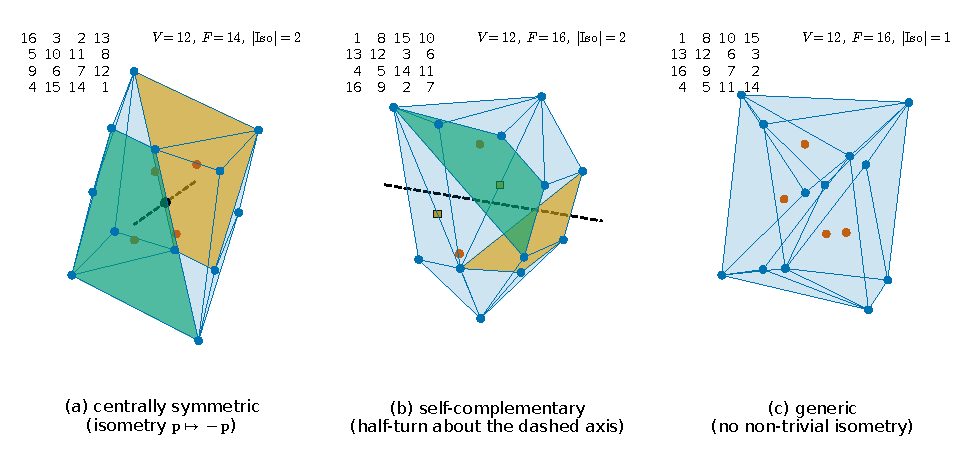
\includegraphics[width=\textwidth]{fig_symmetry.pdf}
\caption{Symmetry types of order-four gems (same viewpoint; strictly interior points are red discs, boundary non-vertex points orange squares; the square is printed above each gem).
(a)~D\"urer's square: a centrally symmetric gem; an antipodal pair of facets $F$ (orange) and $-F$ (green) and the segment joining their centroids through the centre $\mathbf 0$ (dashed).
(b)~A self-complementary, non-associative square (square \#124): the half-turn $\iota$ about the dashed axis swaps the highlighted pair of facets and has no other symmetry.
(c)~A square with no symmetry (square \#102): the gem is chiral, and its mirror image in $z=0$ is the gem of the complement $17-S$.}
\label{fig:symmetry}
\end{figure}

\Cref{fig:pointsets} shows the same three squares as point sets in the height picture: for the associative square the $16$ points form $8$ antipodal pairs $\{\mathbf p,-\mathbf p\}$ whose segments all pass through $O$; for the self-complementary square the half-turn about the dashed horizontal axis exchanges the $8$ pairs, each segment meeting the axis perpendicularly at its midpoint; the third square has no such pairing, in agreement with \Cref{thm:symmetry}.

\begin{figure}[htbp]
\centering
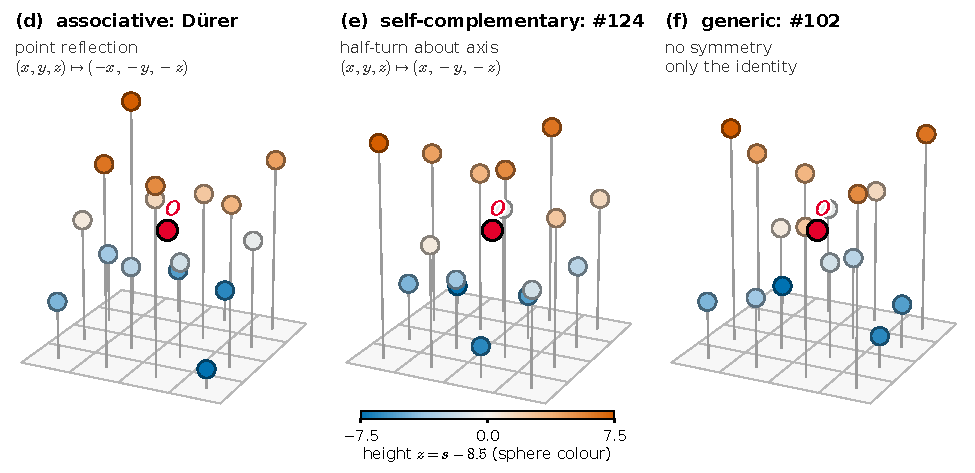
\includegraphics[width=\textwidth]{fig_pointsets.pdf}
\caption{The $16$ points $\mathbf p_{ij}$ as spheres on stems over the floor grid, coloured by height $z$ (same squares and viewpoint as \Cref{fig:symmetry}; $O$ red). (a)~D\"urer's square: the points form $8$ antipodal pairs $\{\mathbf p,-\mathbf p\}$, joined by segments through $O$. (b)~Square \#124: the half-turn $(x,y,z)\mapsto(x,-y,-z)$ about the dashed $x$-axis exchanges $8$ pairs of points, each pair joined by a segment perpendicular to the axis; this gem is chiral. (c)~Square \#102: no non-trivial isometry preserves the point set.}
\label{fig:pointsets}
\end{figure}

\begin{remark}[Classes of order-four squares and vertex counts; exact computation]
\label{rem:classes}
Dudeney's group I consists exactly of the $48$ pandiagonal squares (all broken diagonals sum to $34$), group III of the $48$ associative squares, and group VI of the $304$ self-complementary non-associative squares, whose gems have the half-turn symmetry of \Cref{thm:symmetry}; no order-four square is both pandiagonal and associative.
The gems of the $48$ pandiagonal squares have $11$ to $15$ vertices ($10,20,12,4,2$ gems with $11,\dots,15$), never $16$ and never at most $10$, and each has between one and four strictly interior points.
The $7$ gems with $8$ vertices are squares \#50, \#54, \#672 (group VI) and \#276, \#277, \#494, \#496 (group VIII); none is pandiagonal or associative, and each has $I=B=4$.
\end{remark}

\begin{remark}[Central-symmetry defect]
\label{rem:sigma}
For a convex body $K\subset\R^3$ let $\sigma(K)=\operatorname{vol}\bigl(\tfrac12(K-K)\bigr)/\operatorname{vol}(K)$.
The Brunn--Minkowski inequality gives $\operatorname{vol}(K-K)^{1/3}\ge\operatorname{vol}(K)^{1/3}+\operatorname{vol}(-K)^{1/3}=2\operatorname{vol}(K)^{1/3}$, that is $\sigma(K)\ge1$, and for bodies with non-empty interior equality holds if and only if $K$ and $-K$ are homothetic \cite{schneider2014convex}; since they have equal volume the homothety is a translation, so $\sigma(K)=1$ if and only if $K$ is centrally symmetric.
The defect $\sigma$ is invariant under all isometries including reflections, so $\sigma(\mathcal G(S))=\sigma(\mathcal G(\overline S))$ and $\sigma$ is constant on $D_4$-orbits.
For the $880$ order-four gems, $\sigma$ was computed in exact rational arithmetic from the convex hull of the $256$ pairwise differences of the points (\texttt{anc/central\_symmetry\_defect.py}): $\sigma=1$ for exactly the $48$ associative gems, and $\sigma\in[1057/1018,\,145/88]\approx[1.038,\,1.648]$ for the other $832$, the extremes occurring for squares \#569 and \#218.
\end{remark}

\section{Exact geometry: the order-four gems and the Siamese gems}
\label{sec:results}

All hull computations in this section are exact (integer or rational arithmetic); the methods are in \Cref{sec:appendix}, the scripts and data in the ancillary directory \texttt{anc/}.

\subsection{Geometry of the 880 order-4 gems}
\label{sec:gem-geometry-880}

There are $8$ magic squares of order $3$, all images of the Lo Shu under $D_4$, and $7{,}040$ of order $4$, forming $880$ $D_4$-orbits; the order-four squares are attributed to Fr\'enicle de Bessy (his list was published in 1693) and have been recounted by computer \cite{beck2010enumeration}.
Dudeney sorted them into twelve groups according to the pattern of complementary pairs $(a,17-a)$ \cite{dudeney1917amusements}; we use his groups only as a classical reference partition.
The number $275{,}305{,}224$ of essentially different order-five squares is due to Schroeppel (1973) \cite{gardner1976}; for $n\ge6$ exact counts are, to the author's knowledge, not available (see Trump's compilation \cite{trump2012enumeration}).

For each of the $880$ essentially different order-$4$ magic squares we computed the Magic Gem $\mathcal G(S)$ exactly
(integer facet planes, merged coplanar triangles, rational volumes; \Cref{sec:appendix}); Euler's relation holds for all
$880$ gems.  \Cref{fig:gem-geometry-880} and \Cref{tab:gem-fvectors} summarise the results.

\begin{table}[htbp]
\centering
\caption{Face structure of the $880$ order-$4$ gems by number of hull vertices $V$: number of squares, of distinct
combinatorial types (face lattices up to isomorphism), of distinct exact volumes, and of distinct $f$-vectors $(V,E,F)$.
The full list of the $39$ $f$-vectors with multiplicities is in the ancillary file \texttt{anc/results\_geometry.json}.}
\label{tab:gem-fvectors}
\small
\begin{tabular}{r rrrrrrrrr r}
\toprule
$V$ & 8 & 9 & 10 & 11 & 12 & 13 & 14 & 15 & 16 & all\\
\midrule
squares & 7 & 10 & 103 & 80 & 380 & 106 & 162 & 14 & 18 & 880\\
types   & 4 & 1 & 27 & 32 & 129 & 52 & 85 & 7 & 15 & 352\\
volumes & 4 & 5 & 51 & 33 & 111 & 40 & 65 & 6 & 14 & 155\\
$f$-vectors & 4 & 1 & 6 & 5 & 7 & 5 & 5 & 3 & 3 & 39\\
\bottomrule
\end{tabular}
\end{table}

\paragraph{Vertex counts, $f$-vectors, volumes.}
Between $8$ and all $16$ of the points are hull vertices; $V=12$ is modal ($380/880$).  There are $39$ distinct $f$-vectors,
from $(8,14,8)$ (one gem, square \#54) and $(8,16,10)$ (one gem) to $(16,36,22)$ (nine gems), the modal one being
$(12,26,16)$ ($164$ gems); the multiset of facet sizes (number of triangles, quadrilaterals, \dots) is determined by the
$f$-vector in every case.  The exact volume takes $155$ distinct values, from
$58$ (square \#427) to $292/3$ (square \#379), mean $84.05$.  The denominators are $1,2,3,6$: all three
coordinates of every point are half-odd integers when $n$ is even, so the translate of a gem by $(\frac12,\frac12,\frac12)$ is a
lattice polytope of $\Z^3$ and its volume lies in $\frac16\Z$.
Surface areas range from $116.5$ to $148.6$.

\paragraph{Combinatorial types.}
Two gems have the same combinatorial type if their vertex--facet incidence
structures (equivalently, their face lattices) are isomorphic.  Grouping by a
Weisfeiler--Lehman hash of the bipartite vertex--facet graph and confirming
every group by an explicit graph isomorphism test gives
\[
352\ \text{combinatorial types}
\]
among the $880$ gems (the hash was already exact: no hash class had to be
split).  Their sizes are very uneven; the number of types with $1,2,3,\dots$ members is
\[
\begin{array}{r|rrrrrrrrrrrrrr}
\text{squares per type} & 1&2&3&4&5&6&7&8&10&13&14&16&26&32\\\hline
\text{types} & 93&201&8&20&4&7&4&5&5&1&1&1&1&1
\end{array}
\]
(\Cref{fig:gem-geometry-880}c); the largest type, with $f=(10,22,14)$ (12 triangles,
2 quadrilaterals), is shared by $32$ squares, and the second largest,
$f=(12,24,14)$, by $26$.  The $7$ gems with $8$ vertices fall into $4$ types,
including a single $(8,14,8)$ gem with four triangular and four quadrilateral
faces (square \#54, Fig.~\ref{fig:gem-geometry-880}d) and four
$(8,18,12)$ gems sharing one simplicial type with $12$ triangular faces.  The $18$ gems with all $16$ points
extreme belong to $15$ types.

\paragraph{Congruence classes and injectivity.}
Two gems are \emph{congruent} if an isometry of $\mathbb R^3$ (rotations, reflections, translations) maps one onto the
other; since a distance-preserving bijection between finite point sets extends to an isometry, congruence is decided exactly
by testing for a bijection of hull-vertex sets preserving all integer squared distances (\Cref{sec:appendix}).

\begin{proposition}[class $\to$ gem]
\label{prop:gem-injective}
\begin{enumerate}
\item The $880$ hull-vertex sets are pairwise distinct: the map from
  $D_4$-classes of order-$4$ magic squares to hull-vertex sets (as subsets of
  $\mathbb R^3$) is injective.  (For the full $16$-point sets this is trivial, since the point set determines the
  arrangement.)
\item Up to congruence there are exactly $616$ gems.  The congruence classes
  are precisely the orbits of the complement map $S\mapsto 17-S$, which acts
  on gems as the reflection $z\mapsto -z$: $352$ squares are
  self-complementary (their gems have a non-trivial isometry,
  \Cref{thm:symmetry}) and the other $528$ form $264$ mirror pairs.  No two gems of
  non-complementary squares are congruent, not even as full $16$-point sets.
\end{enumerate}
\end{proposition}

Part (2) is the only failure of injectivity, and it is the expected one: $17-S$ is magic whenever $S$ is, and its gem is the
mirror image of $\mathcal G(S)$ in the plane $z=0$.  The $352$ self-complementary classes are exactly Dudeney's group III (the
$48$ associative squares) together with all $304$ squares of group VI \cite{dudeney1917amusements}.  The coincidence
$352=\#\{\text{types}\}=\#\{\text{self-complementary squares}\}$ is numerical only: the two partitions of the $880$ are different.

\paragraph{Dudeney groups.}
Crossing the hull-vertex count with Dudeney's twelve groups (table in the ancillary files) shows that geometry is only
loosely tied to Dudeney type: every group with more than eight members spans at least three vertex counts and at least $20$
combinatorial types; the $8$-vertex gems occur only in groups VI (three) and VIII (four).


The groups III and VI, the self-complementary ones, have only even vertex counts; this is \Cref{prop:facet-orbits}(3).

\begin{figure}[htbp]
\centering
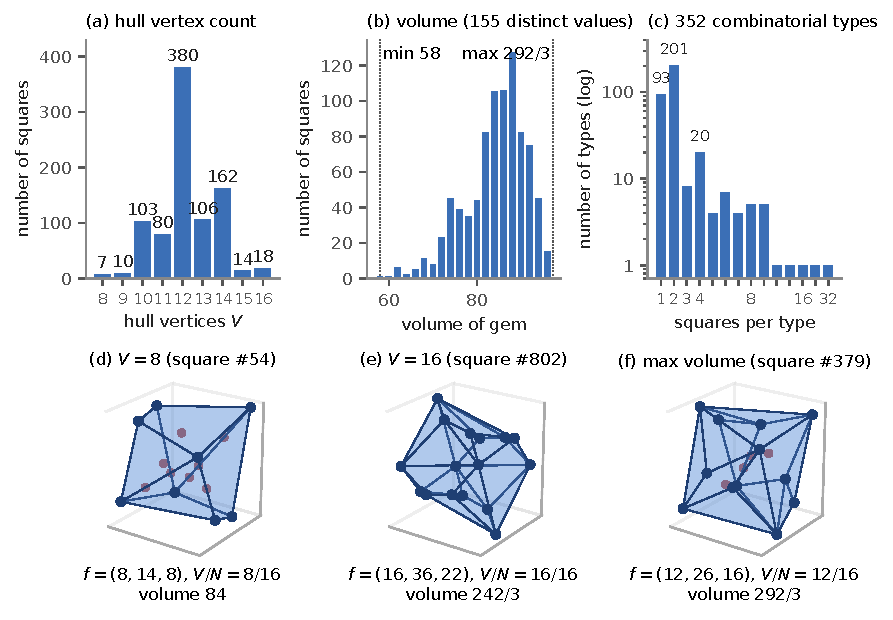
\includegraphics[width=0.9\textwidth]{fig_gem_geometry_880.pdf}
\caption{Geometry of the $880$ order-$4$ Magic Gems.
(a)~Number of hull vertices ($8$ to $16$; modal value $12$).
(b)~Exact hull volume ($155$ distinct values between $58$ and $292/3$).
(c)~Sizes of the $352$ combinatorial types (logarithmic scale): $93$ types occur once, $201$
twice, and one type is shared by $32$ squares.
(d)--(f)~Three extreme gems, drawn with translucent faces after merging
coplanar triangles: the unique $(8,14,8)$ gem (square \#54; its four strictly interior points are red discs and its four boundary non-vertex points orange squares), a gem with all $16$ points extreme
(square \#802, D\"urer's square with its first two rows exchanged and its last two rows exchanged), and the gem of largest
volume (square \#379).}
\label{fig:gem-geometry-880}
\end{figure}

\paragraph{Named squares.}
The gems of the Lo Shu, of D\"urer's square and of the Siamese square of order $5$ have hull fractions $8/9$, $12/16$ and
$12/25$ and exact volumes $18$, $92$ and $830/3$.  D\"urer's own gem is centrally symmetric with twelve vertices, but exchanging its first two rows and
its last two rows (which preserves the magic property) gives a square whose gem has all sixteen points extreme (square \#802,
\Cref{fig:gem-geometry-880}e): the hull-vertex count is a property of the square, not of the Dudeney group or of the
construction method.

% ===========================================================================
\subsection{Extreme points and the bounding box}
\label{sec:box}

Let $B_n=[-\frac{n-1}2,\frac{n-1}2]^2\times[-\frac{N-1}2,\frac{N-1}2]$, a box of volume $(n-1)^2(N-1)$ that depends only on $n$.
The \emph{side lines} of the grid are its first and last rows and columns.

\begin{proposition}[Bounding box and forced vertices]
\label{prop:box}
Let $S$ be any arrangement of order $n\ge2$.
\begin{enumerate}\setlength\itemsep{0pt}\setlength\topsep{2pt}
\item $\mathcal G(S)\subseteq B_n$.
\item The points carrying the entries $1$ and $N$ are the only points on the planes $z=\mp\frac{N-1}2$, and they are vertices of $\mathcal G(S)$.
\item The points over the four corner cells of the grid are vertices.
\item For each of the four side lines, the points over its cells carrying the smallest and the largest entry of that line are vertices.
\end{enumerate}
\end{proposition}

\begin{proof}
(1) $|x_{ij}|,|y_{ij}|\le\frac{n-1}2$ and $1\le s_{ij}\le N$, and $B_n$ is convex.
A point that is the unique maximiser over $\{\mathbf p_{ij}\}$ of a linear functional is a vertex.
(2) The entries are distinct, so $z$ is uniquely minimal where $s=1$ and uniquely maximal where $s=N$.
(3) On the grid the functional $-x+y$ attains its maximum $n-1$ only at the top-left cell, and similarly for the other corners.
(4) Take the left column, where $x=-\frac{n-1}2$ and the other columns have $x\ge-\frac{n-1}2+1$.
For $\varepsilon=1/N$ the functional $-x+\varepsilon z$ has, on points of the column, values greater than $\frac{n-1}2-\frac12$ and, on all other points, values at most $\frac{n-1}2-1+\frac12$; so its maximiser lies in the column and is the point of largest height there, which is unique.
Replacing $\varepsilon z$ by $-\varepsilon z$ gives the point of smallest height, and the other three sides are obtained by applying elements of $D_4$.
\end{proof}

The vertices named in (2)--(4) number at least $4$ and at most $14$; for $n=4$ they number between $4$ and $13$ over the $880$ gems, and nothing more is forced (exact computation, \texttt{anc/box\_and\_classes.py}): the only cells carrying a vertex in all $880$ gems are the four corners, and the only entries that always label a vertex are $1$ and $16$.
In particular $2$ and $N-1$ are not forced: in eight gems the point carrying $2$ is a boundary non-vertex point, for instance for square \#593, $\begin{smallmatrix}4&1&16&13\\5&15&2&12\\14&8&9&3\\11&10&7&6\end{smallmatrix}$, and the complement $17-S$ (the mirror image, \Cref{lem:complement}) has the same property for $15$.
The twelve vertices of a Siamese gem (\Cref{prop:siamese-12}) are its forced vertices.

\Cref{tab:box} gives the volume of the order-four gems as a fraction of $\operatorname{vol}B_4=135$ and the numbers $I$ and $B$ of strictly interior and boundary non-vertex points (exact computation).
Gems fill between $58/135\approx43\%$ and $292/405\approx72\%$ of the box, on average $2219/3564\approx62\%$.
At most four points are strictly interior, while one gem has $I=0$, $B=6$.

\begin{table}[htbp]
\centering
\caption{Order-four gems: volume as a fraction of the box $B_4$ (exact; rounded), by number $V$ of vertices, and numbers of gems with $k$ strictly interior points ($I=k$) and with $k$ boundary non-vertex points ($B=k$).}
\label{tab:box}
\small
\begin{tabular}{r rrrrrrrrr r}
\toprule
$V$ & 8 & 9 & 10 & 11 & 12 & 13 & 14 & 15 & 16 & all\\
\midrule
min & .622 & .588 & .481 & .549 & .430 & .456 & .452 & .498 & .449 & .430\\
mean & .642 & .623 & .631 & .630 & .634 & .614 & .608 & .560 & .536 & .623\\
max & .648 & .667 & .701 & .699 & .721 & .688 & .691 & .615 & .598 & .721\\
\bottomrule
\end{tabular}

\medskip
\begin{tabular}{r rrrrrr}
\toprule
$k$ & 0 & 1 & 2 & 3 & 4 & 6\\
\midrule
gems with $I=k$ & 37 & 32 & 353 & 178 & 280 & 0\\
gems with $B=k$ & 357 & 204 & 257 & 40 & 21 & 1\\
\bottomrule
\end{tabular}
\end{table}

% ===========================================================================
\subsection{Lattice structure and Ehrhart polynomials}
\label{sec:ehrhart}

For even $n$ all coordinates of every $\mathbf p_{ij}$ are half-odd integers, so $Q(S)=\mathcal G(S)+(\frac12,\frac12,\frac12)$ is a lattice polytope; any other lattice translate has the same Ehrhart polynomial $L_S(t)=\#(tQ\cap\Z^3)=\operatorname{vol}(\mathcal G)\,t^3+c_2t^2+c_1t+1$ \cite{beck2007computing}, and $L_S$ is the same for all images $gS$, $g\in D_4$, since $\hat g$ preserves $\Z^3$ up to an integer translation of $Q$.
Writing $\sum_{k\ge0}L_S(k)t^k=(h^*_0+h^*_1t+h^*_2t^2+h^*_3t^3)/(1-t)^4$, the $h^*_i$ are non-negative integers \cite{stanley1980decompositions}, $h^*_0=1$, $\sum h^*_i=6\operatorname{vol}$, and $h^*_3$ is the number of interior lattice points of $Q$ \cite{beck2007computing}.

\emph{Exact computation} (\texttt{anc/ehrhart\_880.py}; lattice points of $tQ$ counted for $t\le6$, the cubic interpolated from $t\le3$ and checked at $t=4,5,6$, with $h^*_3$ checked against the interior count and $\sum h^*_i$ against $6\operatorname{vol}$).
Over the $880$ gems, $h^*_1\in[70,136]$, $h^*_2\in[233,403]$ and $h^*_3\in[34,52]$.
There are $554$ distinct Ehrhart polynomials, against $616$ congruence classes, $352$ combinatorial types, $39$ $f$-vectors and $155$ volumes: congruent gems (complement partners; the reflection $z\mapsto-z$ followed by an integer translation is a unimodular affine map of $\Z^3$) have equal polynomials, but non-congruent gems can share one, and $L_S$ is determined neither by the $f$-vector (it takes several values on $29$ of the $39$ $f$-vectors), nor by the combinatorial type ($81$ of $352$ types), nor by the volume ($104$ of $155$ volumes).
For the Lo Shu square (odd order: the gem itself is a lattice polytope) $L(t)=1+t+13t^2+18t^3$ and $h^*=(1,29,73,5)$; for D\"urer's square $L(t)=1-3t+44t^2+92t^3$ and $h^*=(1,130,377,44)$; the leading coefficients are the volumes $18$ and $92$.

% ===========================================================================
\subsection{Siamese gems have twelve vertices}
\label{sec:siamese-gems}

For the Siamese (de la Loub\`ere) squares of odd order the hull-vertex count
does not grow with $n$.  We computed the gems for $n=3,5,\dots,21$: the Lo Shu
gem has $f=(8,16,10)$, and every Siamese gem with $n\ge5$ has
$f=(12,26,16)$ with $12$ triangular and $4$ quadrilateral facets, so the hull
fraction $12/n^2$ tends to zero.  This is a
theorem, with a short computer-assisted proof.

\begin{proposition}[Siamese gems]
\label{prop:siamese-12}
Let $n=2m+1\ge5$ and let $S$ be the Siamese square of order $n$ ($1$ in the
middle cell of the top row, successive entries one step up and to the right
modulo $n$, one step down when blocked).  Then $\mathcal G(S)$ has exactly $12$
vertices, $26$ edges and $16$ facets ($12$ triangles, $4$ quadrilaterals).
With $0$-indexed cells $(i,j)$ and $c=(n^2+1)/2$, the vertices are the
points over the cells
\[
\begin{array}{lll}
(0,0)\colon c+m+2, & (0,m-1)\colon n^2-1, & (0,m)\colon 1, \\
(0,2m)\colon c+m, & (m-1,0)\colon n^2-m, & (m,0)\colon m+2, \\
(m,2m)\colon n^2-m-1, & (m+1,2m)\colon m+1, & (2m,0)\colon c-m, \\
(2m,m)\colon n^2, & (2m,m+1)\colon 2, & (2m,2m)\colon c-m-2,
\end{array}
\]
i.e.\ the four corners, and on each side of the square the two cells holding
the side's extreme values.  For $n=3$ the same construction gives the Lo Shu
gem, with $8$ vertices (all cells except the centre).
\end{proposition}

\begin{proof}
\emph{Step 1: closed form.}  Write $\langle t\rangle\in\{0,\dots,n-1\}$ for
$t\bmod n$.  We claim $s(i,j)=n\langle i+j-m\rangle+\langle i+2j-2m\rangle+1$.
Indeed, along a run of $n$ consecutive entries the move $(i,j)\to(i-1,j+1)$
fixes $i+j$ and increases $i+2j$ by $1$ modulo $n$, while the ``blocked''
move $(i,j)\to(i+1,j)$ increases both $i+j$ and $i+2j$ by $1$; the entry $1$
sits at $(0,m)$ where both expressions vanish.  Hence by induction the entry
$k$ lies in a cell with $\langle i+j-m\rangle=\lfloor (k-1)/n\rfloor$ and
$\langle i+2j-2m\rangle=\langle k-1\rangle$; since
$(i,j)\mapsto(i+j,\,i+2j)$ is a bijection of $\mathbb Z_n^2$ (determinant
$1$), this determines the cell, which proves the claim.

\emph{Steps 2 and 3 (sketch; details in \Cref{sec:app_siamese}).}  With $m=(n-1)/2$, $x=j-m$, $y=m-i$, the closed form gives
$z=L(x,y)+n\,\zeta(x,y)$ with $L$ affine and
$\zeta=-n\lfloor(x-y+m)/n\rfloor-\lfloor(2x-y+m)/n\rfloor\in\{\pm(n+1),\pm1,0\}$.
The affine bijection $\Phi(x,y,z)=(x,y,(z-L)/n)$ preserves the face lattice and the vertex cells, and
$\Phi(\mathcal G(S))$ is the convex hull of the lattice points of five convex lattice polygons at the five heights $\zeta$:
two triangles $T$, $B=-T$ at $\zeta=\pm(n+1)$, two triangles $U$, $D=-U$ at $\zeta=\pm1$, and a parallelogram $M$ at
$\zeta=0$ (\Cref{fig:siamese-layers}a).  Sixteen explicit planes, eight of them and their images under $(x,y,\zeta)\mapsto
-(x,y,\zeta)$, are shown to support the convex hull of twelve named points $v_1,\dots,v_{12}$---the three corners of $T$ and
of $B$, one corner each of $U$ and $D$, and the four corners of $M$---in facets that close up into a surface with
$(V,E,F)=(12,26,16)$ closed under edge-adjacency, hence all facets (so $P=Q$), and every vertex of every layer polygon satisfies all sixteen inequalities
(\Cref{fig:siamese-layers}b).  These are finitely many polynomial identities and inequalities in $m$, verified exactly for all
integers $m\ge2$ by the script \texttt{siamese\_proof.py}.  Hence $\Phi(\mathcal G(S))=\operatorname{conv}\{v_1,\dots,v_{12}\}$,
and mapping back by $\Phi^{-1}$ gives the statement; for $m=1$ the four triangles degenerate to points and the same argument
gives the $8$-vertex Lo Shu gem.
\end{proof}

\begin{figure}[htbp]
\centering
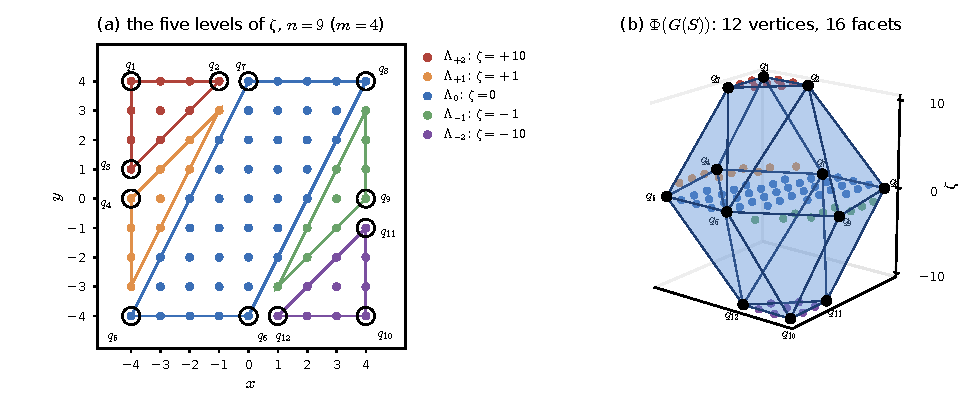
\includegraphics[width=0.88\textwidth]{fig_siamese_layers.pdf}
\caption{The Siamese gem of order $n=9$ after the affine reduction of \Cref{prop:siamese-12}.
(a)~The $81$ cells in the $(x,y)$-plane coloured by the layer value $\zeta\in\{+10,+1,0,-1,-10\}$, with the five lattice
polygons $T,U,M,D,B$ outlined and the twelve vertex cells $v_1,\dots,v_{12}$ circled.
(b)~The reduced polytope $\Phi(\mathcal G(S))=\operatorname{conv}\{(x,y,\zeta)\}$ with its $12$ vertices and $16$ facets
($12$ triangles, $4$ quadrilaterals); the shapes of the layers do not depend on $n$ except through scale, which is why the
combinatorial type is constant for all odd $n\ge5$.}
\label{fig:siamese-layers}
\end{figure}

\section{Discussion and open questions}
\label{sec:discussion}

The Magic Gem is the convex hull of a magic square's height function over the centred grid, and the same polyhedron for all eight $D_4$-images of the square.
The vector picture is exact but easily over-read: the centroid statement belongs to the full point set and holds for every arrangement; the magic conditions are the height-weighted ones; and the hull records only extent (\Cref{sec:balance}).
What the hull does see is symmetry: the complement map acts as a mirror reflection of the gem, and for order four this accounts for all the symmetry there is (\Cref{thm:symmetry}) and for all coincidences between gems (\Cref{prop:gem-injective}).
The coarse invariants, the vertex count (nine values) and the volume ($155$ values), are not well aligned with Dudeney's groups, and the vertex count is a property of the square, not of its group or construction (D\"urer's square versus square \#802).

\paragraph{Hull vertices for larger $n$ (numerical).}
\Cref{tab:vertices} lists the mean number of hull vertices of random arrangements ($10^5$ uniform samples for each $n\le10$, standard error at most $0.010$; Qhull, with the vertex sets of the first $100$ hulls of each batch re-checked in exact integer arithmetic), of the magic squares (exact for $n=3,4$; for $n=5,\dots,8$ the mean over magic squares found by simulated annealing on the sum of squared line deviations, \texttt{anc/sa\_magic.c}), and of the Siamese squares.
The fraction $\mathbb E[V]/n^2$ of random arrangements falls from $0.91$ ($n=3$) to $0.28$ ($n=10$).
At $n=4$ magic gems have slightly more vertices than random ones ($12.23$ against $12.06\pm0.004$); for $n=5,\dots,8$ the annealed means differ from the random means by at most $1.2$ standard errors.
This is a statement about the samples only: at $n=4$, where all $880$ classes are known, the annealer reached every class ($20{,}000$ draws, $10$ to $41$ hits per class, hit-weighted mean $12.24$), but its sampling distribution for $n\ge5$ is unknown and could be biased towards easily reached squares.
The Siamese value $12$ is thus atypical: it stays constant while the means grow (for $n=7$ the smallest vertex count among $8000$ annealed squares is $14$, for $n=8$ it is $16$ among $2400$).

\begin{table}[htbp]
\centering
\caption{Mean number of hull vertices (numerical except where marked exact). Random: uniform random arrangements; magic: exact for $n=3,4$, annealing samples of $59{,}993$, $24{,}000$, $8{,}000$, $2{,}400$ squares for $n=5,\dots,8$ (standard errors $0.007$, $0.013$, $0.025$, $0.054$); Siamese: exact.}
\label{tab:vertices}
\small
\begin{tabular}{l rrrrrrrr}
\toprule
$n$ & 3 & 4 & 5 & 6 & 7 & 8 & 9 & 10\\
\midrule
random, $\mathbb E[V]$ & 8.22 & 12.06 & 15.39 & 18.39 & 21.08 & 23.53 & 25.79 & 27.91\\
magic & 8 (exact) & 12.23 (exact) & 15.38 & 18.41 & 21.08 & 23.56 & -- & --\\
Siamese & 8 & -- & 12 & -- & 12 & -- & 12 & --\\
\bottomrule
\end{tabular}
\end{table}

\paragraph{Open questions.}
\begin{enumerate}\setlength\itemsep{1pt}
\item \emph{Order five.} By Schroeppel's enumeration there are $275{,}305{,}224$ essentially different squares of order $5$ \cite{gardner1976}; an exact hull computation for each is feasible. How many combinatorial types occur, what is the modal $f$-vector, and is the complement map again the only source of congruence? By \Cref{prop:selfcomp} the self-complementary squares of odd order are exactly the associative ones, so every symmetric gem of order five is centrally symmetric.
\item \emph{Symmetry in general.} Is $\operatorname{Iso}(\mathcal G(S))$ generated by the complement symmetry for every magic square of every order, as it is for order four?
\item \emph{Bounded hull-vertex counts.} Siamese gems have twelve vertices for every odd $n\ge5$ because, affinely, they are hulls of five lattice polygons whose shapes do not depend on $n$ (\Cref{prop:siamese-12}). Do the LUX, Strachey or diagonal-complement constructions have the same property, and is the fraction of vertices for a uniformly random magic square of large order bounded away from zero?
\item \emph{Other square families.} The construction applies verbatim to semi-magic, pandiagonal and Franklin squares \cite{loly2007franklin}; the statements of \Cref{prop:signed_mass} already cover the semi-magic case. The gems of these families have not been examined.
\end{enumerate}


\bibliographystyle{plain}
\bibliography{references}

\appendix
\section{Computational methods}
\label{sec:appendix}

\paragraph{Hardware and software.}
All computations were run on an Apple M4 Max (16 cores, 128\,GB) under macOS, with Python 3.9.6, NumPy 2.0.2, SciPy 1.13.1 (Quickhull only seeds the exact hull computation) and NetworkX 3.2.1.
The scalar identities of \Cref{sec:balance} (the value $n^2(n^4-1)/12$ for the semi-magic squares and the product-of-inertia statistics over the $880$ classes) were checked in exact integer arithmetic.

\paragraph{Exact hulls and their classification.}
Doubling all coordinates makes every point of a gem an integer vector.
Facet planes are recovered from an initial Quickhull triangulation as primitive integer equations, coplanar triangles are merged into faces, vertices are the points on at least three facet planes, edges are vertex pairs sharing two facets, and volumes are exact rationals; Euler's relation $V-E+F=2$ is checked for every gem.
Combinatorial types are the isomorphism classes of the bipartite vertex--facet incidence graphs, grouped by a Weisfeiler--Lehman hash and confirmed by explicit isomorphism tests.
Isometry groups (\Cref{thm:symmetry}) are computed exactly as follows: the vertex set $V$ ($k$ points, doubled integer coordinates) is centred by $\mathbf q\mapsto k\mathbf q-\sum V$; an isometry of $V$ is an orthogonal map fixing the origin, determined by the images of three linearly independent vertices, which are searched among the vertices with the same squared norm and mutual inner products; each candidate is accepted only if the induced bijection of $V$ preserves all pairwise integer squared distances. Congruence is decided exactly by testing for a bijection of hull-vertex sets preserving all integer squared distances (grouping by the sorted distance multiset, then an edge-labelled graph isomorphism), with a floating-point Kabsch superposition as a cross-check.
For the Siamese proof (\Cref{prop:siamese-12}, \Cref{sec:app_siamese}) the finitely many polynomial identities and inequalities in $m$ are verified by exact integer polynomial arithmetic, an inequality $p(m)>0$ for all integers $m\ge2$ being certified by positivity of the coefficients of $p(2+t)$ or, failing that, by exact evaluation up to a Cauchy root bound.

\paragraph{Reproducibility.}
The scripts for every table and figure and the JSON files containing all reported numbers are provided as ancillary files in the directory \texttt{anc/}, with a \texttt{README} listing the commands that regenerate them. Squares are numbered $0,\dots,879$ in the order of \texttt{anc/squares880.txt}.
The web application at \url{https://kylemath.github.io/MagicGemWebpage/} displays the $880$ essentially different order-four squares and renders the gem of a selected one.


\section{Siamese gems: the remaining steps of the proof}
\label{sec:app_siamese}

We continue the proof of \Cref{prop:siamese-12} from the closed form $s(i,j)=n\langle i+j-m\rangle+\langle i+2j-2m\rangle+1$.

\emph{Step 2: affine reduction to five layers.}  In gem coordinates $x=j-m$, $y=m-i$, with $\langle t\rangle=t-n\lfloor t/n\rfloor$,
\[
z=\underbrace{n(x-y+m)+(2x-y+m)+1-\tfrac{n^2+1}{2}}_{L(x,y)\ \text{affine}}+\;n\,\zeta(x,y),\quad
\zeta:=-n\Big\lfloor\tfrac{x-y+m}{n}\Big\rfloor-\Big\lfloor\tfrac{2x-y+m}{n}\Big\rfloor .
\]
The map $\Phi(x,y,z)=(x,y,(z-L(x,y))/n)$ is an affine bijection, so $\Phi(\mathcal G(S))=\operatorname{conv}\{(x,y,\zeta)\}$ has the
same face lattice and vertex cells as $\mathcal G(S)$.  In the box $|x|,|y|\le m$ both floors lie in $\{-1,0,1\}$, the pairs
$(-1,1),(-1,0)$ and, by the central symmetry $\zeta(-x,-y)=-\zeta(x,y)$, $(1,-1),(1,0)$ are impossible, so $\zeta$ takes the
five values $\pm(n+1),\pm1,0$ on the lattice points of five convex lattice polygons (\Cref{fig:siamese-layers}a):
$T=\operatorname{conv}\{(-m,m),(-1,m),(-m,1)\}$ at $\zeta=n+1$ (cut out by $y\ge x+m+1$),
$U=\operatorname{conv}\{(-m,1-m),(-m,0),(-1,m-1)\}$ at $\zeta=1$ (by $2x+m+1\le y\le x+m$),
$M=\operatorname{conv}\{(-m,-m),(0,m),(m,m),(0,-m)\}$ at $\zeta=0$ (by $|y-2x|\le m$), and $D=-U$, $B=-T$ at $\zeta=-1,-(n+1)$.

\emph{Step 3: the twelve points and sixteen planes.}  Let
$v_1=(-m,m,n{+}1)$, $v_2=(-1,m,n{+}1)$, $v_3=(-m,1,n{+}1)$, $v_4=(-m,0,1)$,
$v_5=(-m,-m,0)$, $v_6=(0,-m,0)$, $v_7=(0,m,0)$, $v_8=(m,m,0)$, $v_9=(m,0,-1)$,
$v_{10}=-v_1$, $v_{11}=-v_3$, $v_{12}=-v_2$ (the cells listed in the statement), and consider the inequalities
\begin{align*}
&(1)\ \zeta\le 2m+2, \qquad (2)\ y\le m, \qquad (3)\ x\ge -m, \qquad (8)\ -2y+\zeta\le 2m,\\
&(4)\ -2(m{+}1)x+(2m{+}1)y-m\zeta\le m(2m{+}1),\\
&(5)\ 2(m{+}1)x-2(m{+}1)y+(2m{+}1)\zeta\le 2m(m{+}1),\\
&(6)\ 2m(m{+}2)x-(2m^2{+}2m{-}1)y+m(2m{+}1)\zeta\le m(2m^2{+}2m{-}1),\\
&(7)\ 2mx-y+m\zeta\le m(2m{-}1),
\end{align*}
together with their images $(1')$--$(8')$ under $(x,y,\zeta)\mapsto-(x,y,\zeta)$; let $Q$ be the polyhedron they define.
The script \texttt{siamese\_proof.py} verifies, as polynomial identities and inequalities in $m$ valid for all integers $m\ge2$
(\Cref{sec:appendix}): (a)~every vertex of $T,U,M,D,B$ at its height satisfies all $16$ inequalities, so
$\Phi(\mathcal G(S))\subseteq Q$; (b)~each plane contains exactly the following $v$'s, all others lying strictly inside:
\[
\begin{array}{llll}
(1)\colon v_1v_2v_3, & (2)\colon v_1v_2v_8v_7, & (3)\colon v_1v_3v_5v_4, & (4)\colon v_1v_4v_7,\\
(5)\colon v_2v_3v_6, & (6)\colon v_2v_6v_9, & (7)\colon v_2v_8v_9, & (8)\colon v_3v_5v_6,
\end{array}
\]
with centrally symmetric lists for $(1')$--$(8')$; (c)~the quadrilaterals are in convex position in the cyclic order given, so
the $16$ face polygons have $26$ distinct edges, each shared by exactly two polygons; (d)~each $v_k$ lies on three planes with
independent normals.  By (b) each plane supports $P:=\operatorname{conv}\{v_1,\dots,v_{12}\}$ in a facet with the stated vertices;
by (c) this family of facets is closed under edge-adjacency, and since the facet-adjacency graph of a $3$-polytope is connected
these are all the facets, so $P=Q$.  With (a), $P\subseteq\Phi(\mathcal G(S))\subseteq Q=P$, whose vertex set is
$\{v_1,\dots,v_{12}\}$ by (d); mapping back by $\Phi^{-1}$ gives the statement, with $(V,E,F)=(12,26,16)$ read off from (b)--(c).
For $m=1$ the triangles degenerate to points and the same argument gives the $8$-vertex Lo Shu gem.


\end{document}
